\documentclass[11pt, a4paper]{article}
\usepackage[utf8]{inputenc}
\usepackage{amsmath,setspace,geometry}
\usepackage{amsthm}
\usepackage{amsfonts}
\usepackage{mathtools}
\mathtoolsset{showonlyrefs}
\usepackage[shortlabels]{enumitem}
\usepackage{rotating}
\usepackage{pdflscape}
\usepackage{graphicx}
\usepackage{bbm}
\usepackage[dvipsnames]{xcolor}
\usepackage[colorlinks=true, linkcolor= RawSienna, citecolor = RawSienna, filecolor = RawSienna, urlcolor = RawSienna, hypertexnames = true, backref = page]{hyperref}
\usepackage[]{natbib} 
\bibpunct[:]{(}{)}{,}{a}{}{,}
\geometry{left = 1.0in,right = 1.0in,top = 1.0in,bottom = 1.0in}
\usepackage[english]{babel}
\usepackage{float}
\usepackage{caption}
\usepackage{subcaption}
\usepackage{tikz}
\usepackage{booktabs}
\usepackage{pdfpages}
\usepackage{threeparttable}
\usepackage{framed}
\usepackage{comment}
\usepackage{lscape}
\usepackage{bm}
\setstretch{1.4}
%\usepackage[tablesfirst,nolists]{endfloat}

\usepackage[T1]{fontenc}
\usepackage{mlmodern}  % 太いComputer Modern
% MLmodernのバグを修正: cf. https://tex.stackexchange.com/questions/646333/size-of-integral-symbol-in-section-header-with-mlmodern
\DeclareFontFamily{OMX}{mlmex}{}
\DeclareFontShape{OMX}{mlmex}{m}{n}{<->mlmex10}{} 
\usepackage{tgtermes} % 数式以外の欧文をTXフォントで上書き

\newtheorem{theorem}{Theorem}
\newtheorem{assumption}{Assumption}
\newtheorem{lemma}{Lemma}
\newtheorem{definition}{Definition}
\newtheorem{proposition}{Proposition}
\newtheorem{claim}{Claim}
\newtheorem{corollary}{Corollary}
\newtheorem{example}{Example}
\DeclareMathOperator{\rank}{rank}

\theoremstyle{remark}
\newtheorem{remark}{Remark}

\title{Revisiting the identification of conduct parameters in homogeneous goods markets}
\author{Yuri Matsumura\thanks{Department of Economics, Rice University. Email: \href{mailto:yuri.matsumura23@gmail.com}{yuri.matsumura23@gmail.com}} \and Suguru Otani \thanks{Market Design Center, Department of Economics, University of Tokyo. Email: \href{mailto:suguru.otani@e.u-tokyo.ac.jp}{suguru.otani@e.u-tokyo.ac.jp}
}}

\begin{document}

\maketitle
\begin{abstract}
    We revisit the identification of the conduct parameter in homogeneous goods markets.
    \citet{lau1982identifying} shows that the conduct parameter cannot be identified if and only if the demand function is separable but not a specific functional form.
    However, we provide a novel characterization of non-identification and show that the statement in \citet{lau1982identifying} is incorrect.
    Specifically, we show that the class of inverse demand functions that lead to identification is much broader than \citet{lau1982identifying} considers.
    Our result also emphasizes the insight of \citet{bresnahan1982oligopoly} that the demand rotation instrument is crucial for the identification of the conduct parameter.
\end{abstract}

\noindent\textbf{Keywords:} Conduct parameters, Homogenous Goods Market, Identification
\vspace{0in}
\newline
\noindent\textbf{JEL Codes:} C5, C13, L1

\bigskip





\section{Introduction}
Measuring competitiveness is an important task in the empirical industrial organization literature.
The conduct parameter approach is one of the useful approaches to measure competitiveness.
However, the parameter cannot be directly measured from data because data generally lack information about marginal costs.
Therefore, researchers endeavor to identify and estimate conduct parameters.

In homogeneous goods markets, \cite{bresnahan1982oligopoly} considers the identification of conduct parameter and marginal cost function in linear demand and linear marginal cost model.
\citet{bresnahan1982oligopoly} finds that when the researcher can obtain a type of demand shifter, called demand rotation instrument, which changes the slope and intercept of the inverse demand function, conduct parameter and marginal cost parameter can be identified.
Recently, \citet{matsumura2023resolving} provide a detailed condition for the identification.
Then, \citet{lau1982identifying} considers a more general setting and shows that the conduct parameter is not identified if and only if the demand function is separable, except a specific functional form.
As introducing demand rotation instrument makes a inverse demand function non-separable, this result implies that the insight of \citet{bresnahan1982oligopoly} is crucial for the identification of conduct parameter in homogeneous goods markets even in a general setting.


The contributions of this paper are as follows. 
First, we point out that the proof of \citet{lau1982identifying} has some problems.
The key argument in his proof is that non-identification implies that there is a transformation between the equilibrium condition under two different models.
In other words, given an equilibrium quantity under a conduct parameter and a marginal cost function, we can construct a transformation that transforms the equilibrium condition under the given conduct parameter and marginal cost function into the equilibrium condition under another conduct parameter and another marginal cost function that satisfies the equilibrium quantity in both models.
This implies that we have two distinct pairs of a conduct parameter and a marginal cost that lead to observable equivalent equilibrium.
However, the way of finding such transformation is incorrect.

Next, to avoid the problem, we provide a novel characterization of non-identification to construct a transformation that can connect the equilibrium condition under two different models.
To make the transformation work, we can restrict the functional form of the inverse demand function.
Surprisingly, the resulting class of inverse demand functions implied by non-identification is the set of inverse demand functions that are separable but more restrictive functional form.
Additionally, we find that the class of inverse demand functions also works as a sufficient condition for non-identification.
Therefore, the class of inverse demand functions that lead to identification is much broader than \citet{lau1982identifying} considers.

\section{Setting}\label{sec:setting}
Consider a homogeneous product market with a representative 













Consider a homogeneous product market with the aggregate inverse demand and aggregate marginal cost function as $P(Q, X^{d})$ and $MC(Q, X^{s})$ where $X^{d}$ and $X^{s}$ are the vector of exogenous variables.
Let $K_d$ and $K_s$ be the dimension of $X^{d}$ and $X^{s}$, respectively.
We call $X^{d}$ demand shifters and $X^{s}$ cost shifters, and assume the following:
\begin{assumption}\label{assumption:exclusive_shifters}
    The demand shifter $X^{d}$ and the cost shifter $X^{s}$ are exclusive; that is, there is no common variable in $X^{d}$ and $X^{s}$, and $X^{d}$ affects the demand function but not the marginal cost function, and $X^{s}$ affects the marginal cost function but not the demand function; for all $i = 1, \ldots, K_d$ and $j = 1, \ldots, K_s$,
    \begin{align}
        \frac{\partial P}{\partial X^{d}_{i}}(Q, X^{d}) \ne 0 \quad \text{and} \quad \frac{\partial MC}{\partial X^{s}_{j}}(Q, X^{s}) \ne 0,\\
        \frac{\partial P}{\partial X^{s}_{j}}(Q, X^{d}) = 0 \quad \text{and} \quad \frac{\partial MC}{\partial X^{d}_{i}}(Q, X^{s}) = 0.
    \end{align}
\end{assumption}
We can also include some common variables in $X^{d}$ and $X^{s}$, but in that case, we still have some variable that exclusively affects the demand function and the marginal cost function.
\citet{lau1982identifying} also imposes the following restriction on the inverse demand and the marginal cost function:
\begin{assumption}\label{assumption:twice_differentiable}
    The inverse demand and the marginal cost function are twice continuously differentiable.
\end{assumption}

The equilibrium quantity $Q^e$ is defined as the solution to the following equation:
\begin{align}
    F(Q^e, X^{d}, X^{s}; \theta, MC) \equiv P(Q^e, X^{d}) + \theta Q^e\frac{\partial P}{\partial Q}(Q^e, X^{d}) - MC(Q^e, X^{s}) = 0, \label{eq:foc}
\end{align}
where $\theta$ is called the conduct parameter.
Depending on the value of $\theta$, the relation can nest the equilibrium condition of several models, such as perfect competition ($\theta=0$) and Cournot competition ($\theta=1/N$).

\citet{lau1982identifying} does not impose any further restrictions, but we are interested in the point identification of the conduct parameter and the marginal cost function, and hence it is natural to assume that the equilibrium quantity exists and is unique, which needs the following additional assumption:
\begin{assumption}\label{assumption:unique_equilibrium}
    Given an inverse demand function, a conduct parameter, and a marginal cost function, and given $X^{d}$ and $X^{s}$,
    \begin{align}
        \frac{\partial F}{\partial Q}(Q^{e}, X^{d}, X^{s}; \theta, MC) \ne 0 \text{ and } \left| \frac{\partial F}{\partial Q}(Q^{e}, X^{d}, X^{s}; \theta, MC)\right| < \infty. 
    \end{align}
\end{assumption}




\subsection{Non-identification of the conduct parameter and the marginal cost function}\label{sec:definition_identification}

Suppose that the researcher observes the aggregate price $P$ and the aggregate quantity $Q$, and the vector of exogenous variables $X^{d}$ and $X^{s}$.
Then, \citet{lau1982identifying} considers the identification problem of the conduct parameter and the marginal cost function.
Based on the exogenous variables, the researcher can identify the reduced form of the equilibrium quantity $Q^e = h_q(X^{d}, X^{s})$.
Given the inverse demand function, the reduced form of the equilibrium price is $P$, defined as $h_p(X^{d}, X^{s})$, is also identified.
We put this fact as an assumption:
\begin{assumption}\label{assumption:reduced_form_identification}
    The reduced form of the equilibrium quantity $Q^e = h_q(X^{d}, X^{s})$ and the reduced form of the equilibrium price $P^e = h_p(X^{d}, X^{s})$ are identified from the data on price, quantity, and other exogenous variables.
\end{assumption}

\citet{lau1982identifying} takes an indirect approach and specifies the conditions under which the model is not identified.
The definition of non-identification is as follows:
\begin{definition}\label{def:non_identification}
    Non-identification implies for any $X^{d}$ and $X^{s}$,
    \begin{align}
    & P(Q^e, X^{d}) + \theta Q^e\frac{\partial P}{\partial Q}(Q^e, X^{d}) = MC(Q^e, X^{s}) ,  \label{eq:foc_alpha}\\
    & P(Q^e, X^{d}) + \theta^{*} Q^e\frac{\partial P}{\partial Q}(Q^e, X^{d}) = MC^{*}(Q^e, X^{s}),\label{eq:foc_beta}
    \end{align}
    where $\theta \neq \theta^{*}$, $MC \ne MC^{*}$, and the equilibrium quantity $Q^e$ has a reduced form functions $Q^e = h_q(X^{d}, X^{s})$ and $Q^e = h_q^{*}(X^{d}, X^{s})$ defined by \eqref{eq:foc_alpha} and \eqref{eq:foc_beta} respectively are identical.
\end{definition}
In other words, given two distinct pairs of the conduct parameter and the marginal cost, the equilibrium quantity $Q^e$ solves the equilibrium condition for both pairs.
Non-identification asks the following question: given an inverse demand function, is it possible to find two distinct pairs of a conduct parameter and a marginal cost that lead to observable equivalent equilibrium?

Then, \citet{lau1982identifying} finds that the separability of the inverse demand function and non-identification are equivalent.
\begin{theorem}\label{theorem_lau}
    Given Assumption \ref{assumption:twice_differentiable} and Assumption \ref{assumption:unique_equilibrium},
    the conduct parameter $\theta$ cannot be identified from data on price, quantity, and other exogenous variables alone if and only if the industry inverse demand function is separable in $X^{d}$, that is,
    \begin{align}
        P(Q, h(X^{d})), \label{eq:demand_separable}
    \end{align}
    but not take the form, 
    \begin{align}
        P(Q, h(X^{d})) = Q^{-1/\theta}h(X^{d}) + k(Q). \label{eq:identification_separable}
    \end{align}
\end{theorem}
The inverse demand function satisfies \eqref{eq:demand_separable} has weak separability defined in \citet{goldmanNote1964}.
Additionally, when the demand shifter is a scalar, the function $h(X^{d})$ is regarded as a single variable depending on $X^{d}$.
Thus, the theorem implies that when the demand shifter is a scalar, the conduct parameter can be identified only when the inverse demand function takes the form \eqref{eq:identification_separable}.
Because Theorem \ref{theorem_lau} derives the condition for non-identification, the shape of the inverse demand function and the dimension of the demand shifter are important for the identification.



\section{We can identify the conduct parameter even when the demand function is separable}\label{sec:identification_example}





We first show that the identification result in \citet{lau1982identifying} is incorrect by providing a counterexample where a separable demand function induces identification.

The intuition is the following.
Consider a linear demand with a demand rotation instrument, given by
\begin{align}
    P(Q, X^{d}) = \alpha_0 - \alpha_1Q + \alpha_2X^{d} + \alpha_3QX^{d}. \label{eq:demand_counterexample}
\end{align}
Because the demand shifter is a scalar, the inverse demand function satisfies \eqref{eq:demand_separable}.
Here, the demand shifter is works as a demand rotation instrument introduced in \citet{bresnahan1982oligopoly} to identify the conduct parameter.
\citet{bresnahan1982oligopoly} considers the linear demand and the linear marginal cost function, but let's see why the demand rotation instrument works even when a more general environment.
Suppose that the true conduct is the perfect competition, that is, $\theta = 0$ and the alternative conduct is the monopoly, that is, $\theta^{*} = 1$.
The true and alternative marginal cost functions are also given as linear functions.

Figure \ref{fig:identification_example} illustrates the intuition.
Figure \ref{fig:identification_example_step_1} illustrates the non-identification result.
When the true conduct is the perfect competition, the equilibrium point is $E$, but the marginal revenue under the monopoly, $MR^{*}$, and the marginal cost $MC^{*}$ leads to the same equilibrium point $E$.
Now, let's consider the change in the demand rotation instrument.
In Figure \ref{fig:identification_example_step_2}, the demand rotation changes the intercept and slope of the demand function without changing the equilibrium point under the true model.
Then, under the monopoly, the new equilibrium point is $E^{*}$, which is different from $E$ and hence the observable equivalence is violated.

When $MC^{*}$ leads to the same equilibrium point $E$ after the change in the demand rotation, $MC^{*}$ should shift as in Figure \ref{fig:identification_example_step_3}.
However, this cannot be done by the cost shifter because if this does by a cost shifter, it also changes the true marginal cost function $MC$.
Therefore, the shift in $MC^{*}$ should correlate with the change in the demand rotation, which implies that $MC^{*}$ should be a function of the demand shifter.
This is impossible because it violates Assumption \ref{assumption:exclusive_shifters}.

Here, we consider the case $MC^{*}$ is also a linear function.
Non-identification requires to find two distinct pairs of conduct parameter and marginal cost function that lead to the same equilibrium quantity, and hence there is a possibility that under non-linear $MC$ and $MC^{*}$, $MC^{*}$ can achieve observable equivalence without depending on the demand shifter.
However, as we will see later, this is impossible under the inverse demand and the same intuition applies.

\begin{figure}[p!]
    \begin{center}
        \begin{subfigure}[b]{0.45\textwidth}
            \centering
            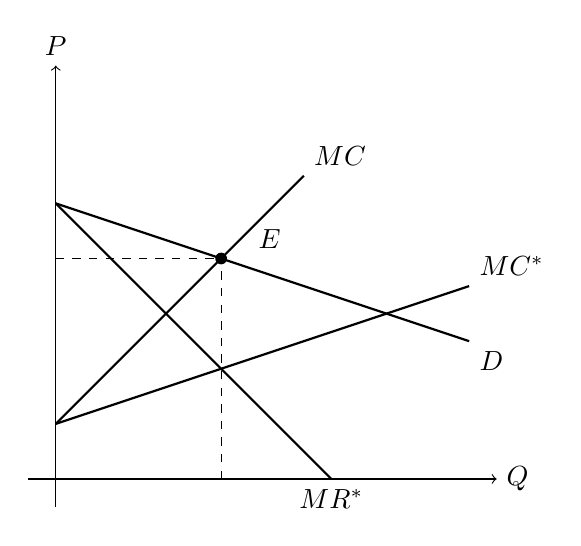
\begin{tikzpicture}[scale = 0.7]
                % Axes
                \draw[->] (-0.5,0) -- (8,0) node[right] {$Q$}; % Horizontal axis
                \draw[->] (0,-0.5) -- (0,7.5) node[above] {$P$}; % Vertical axis

                % Demand Curve (D_1) - passes through (0,5), (3,4), and (7.5,2.5)
                \draw[thick] (0,5) -- (7.5,2.5) node[below right] {$D$};
                % Marginal Revenue (MR_1) - passes through (0,5), (3,2), and (5,0)
                \draw[thick] (0,5) -- (5,0) node[below] {$MR^{*}$};

                % Supply Curve under competition (S^c) - passes through (0,1), (3,4), and (4.5,5.5)
                \draw[thick] (0,1) -- (4.5,5.5) node[above right] {$MC$};

                % Supply Curve under monopoly (S^m) - passes through (0,1), (3,2), and (7.5,3.5)
                \draw[thick] (0,1) -- (7.5,3.5) node[above right] {$MC^{*}$};

                % Equilibrium point (E_1) - intersection of D_1 and S^c at (3,4)
                \node[circle, fill, inner sep=1.5pt] (E1) at (3,4) {};
                \node[above right] at (E1) {$\quad E$};
                \draw[dashed] (3,0) -- (3,4);
                \draw[dashed] (0,4) -- (3,4);
            \end{tikzpicture}
            \caption{Step 1: Observable equivalence holds.}
            \label{fig:identification_example_step_1}
        \end{subfigure}
        \hfill
        \begin{subfigure}[b]{0.45\textwidth}
            \centering
            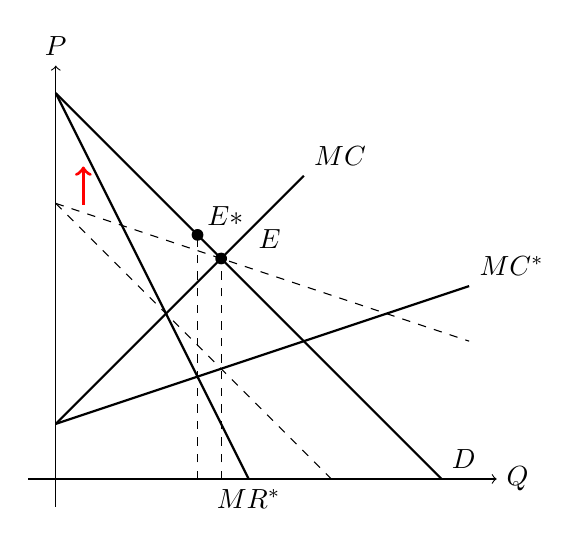
\begin{tikzpicture}[scale = 0.7]
                % Axes
                \draw[->] (-0.5,0) -- (8,0) node[right] {$Q$}; % Horizontal axis
                \draw[->] (0,-0.5) -- (0,7.5) node[above] {$P$}; % Vertical axis

                % Demand Curve (D_1) - passes through (0,5), (3,4), and (7.5,2.5)
                \draw[dashed] (0,5) -- (7.5,2.5) ;
                % Marginal Revenue (MR_1) - passes through (0,5), (3,2), and (5,0)
                \draw[dashed] (0,5) -- (5,0);


                % Shifted Demand Curve (D_1 shifted)
                \draw[thick] (0,7) -- (7,0) node[above right] {$D$};
                % Shifted MR (MR_1 shifted)
                \draw[thick] (0,7) -- (3.5,0) node[below] {$MR^{*}$};

                \draw[-<, very thick, red] (0.5,5) to[out=270,in=90] (0.5,5.5);


                % Supply Curve under competition (S^c) - passes through (0,1), (3,4), and (4.5,5.5)
                \draw[thick] (0,1) -- (4.5,5.5) node[above right] {$MC$};

                % Supply Curve under monopoly (S^m) - passes through (0,1), (3,2), and (7.5,3.5)
                \draw[thick] (0,1) -- (7.5,3.5) node[above right] {$MC^{*}$};

                % Equilibrium point (E_1) - intersection of D_1 and S^c at (3,4)
                \node[circle, fill, inner sep=1.5pt] (E1) at (3,4) {};
                \node[above right] at (E1) {$\quad E$};
                \draw[dashed] (3,0) -- (3,4);

                % Equilibrium point (E_2) - intersection of D_1 and S^c at (7/2,9/2)
                \node[circle, fill, inner sep=1.5pt] (E2) at (18/7,7 - 18/7) {};
                \node[above right] at (E2) {$E{*}$};
                \draw[dashed] (18/7,0) -- (18/7,7 - 18/7);
            \end{tikzpicture}
            \caption{Step 2: Demand rotation changes $D$ and $MR^{*}$}
            \label{fig:identification_example_step_2}
        \end{subfigure}
        \begin{subfigure}[b]{0.5\textwidth}
            \centering
            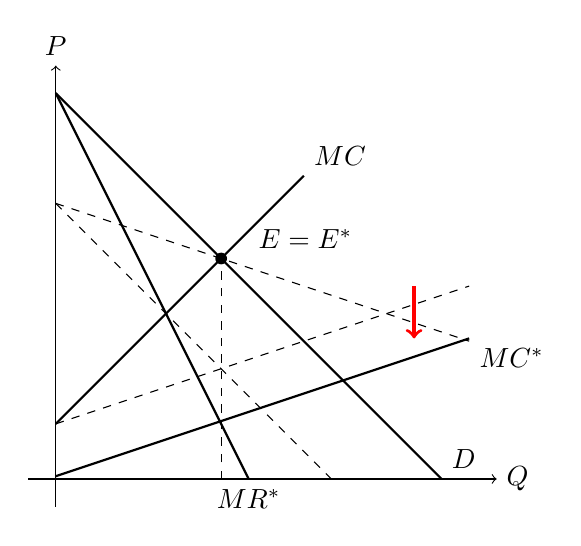
\begin{tikzpicture}[scale = 0.7]
                % Axes
                \draw[->] (-0.5,0) -- (8,0) node[right] {$Q$}; % Horizontal axis
                \draw[->] (0,-0.5) -- (0,7.5) node[above] {$P$}; % Vertical axis

                % Demand Curve (D_1) - passes through (0,5), (3,4), and (7.5,2.5)
                \draw[dashed] (0,5) -- (7.5,2.5) ;
                % Marginal Revenue (MR_1) - passes through (0,5), (3,2), and (5,0)
                \draw[dashed] (0,5) -- (5,0);

                % Shifted Demand Curve (D_1 shifted)
                \draw[thick] (0,7) -- (7,0) node[above right] {$D$};
                % Shifted MR (MR_1 shifted)
                \draw[thick] (0,7) -- (3.5,0) node[below] {$MR^{*}$};

                % Supply Curve under competition (S^c) - passes through (0,1), (3,4), and (4.5,5.5)
                \draw[thick] (0,1) -- (4.5,5.5) node[above right] {$MC$};

                % Supply Curve under monopoly (S^m) - passes through (0,1), (3,2), and (7.5,3.5)
                \draw[dashed] (0,1) -- (7.5,3.5);
                \draw[->, very thick, red] (6.5,3.5) -- (6.5,2.55);

                % Supply Curve under monopoly (S^m) - passes through (0,1), (3,2), and (7.5,3.5)
                \draw[thick] (0,0.05) -- (7.5,2.55) node[below right] {$MC^{*}$};

                % Equilibrium point (E_1) - intersection of D_1 and S^c at (3,4)
                \node[circle, fill, inner sep=1.5pt] (E1) at (3,4) {};
                \node[above right] at (E1) {$\quad E = E^{*}$};
                \draw[dashed] (3,0) -- (3,4);

            \end{tikzpicture}
            \caption{Step 3: $MC^{*}$ should change along with the demand rotation to keep $E = E^{*}$.}
            \label{fig:identification_example_step_3}
        \end{subfigure}
    \end{center}
    \caption{Intuition of the role of demand rotation instrument and identification}
    \label{fig:identification_example}
    \vspace{2mm}
    \footnotesize
    Note: The figures illustrate the intuition of how the demand rotation instrument works to identify the conduct parameter.
    $MC$ is the true marginal cost function, and $MC^{*}$ is the marginal cost function that rationalizes the monopoly conduct.
    Step 1 illustrates monopoly and perfect competition are observationally equivalent.
    In step 2, the demand rotation changes the intercept and slope of the demand function without changing the equilibrium point under perfect competition, but changes the equilibrium point under monopoly.
    Step 3 illustrates that to keep the equilibrium point under monopoly, $MC^{*}$ should change along with the demand rotation, which is impossible because the marginal cost function is independent of the demand shifter.
\end{figure}



\section{Characterization of non-identification}\label{sec:non-identification_characterization}





\begin{proposition}\label{proposition:non-identification_charaterization}
    Non-identification implies that for any $Q^e$, $X^{d}$, and $X^{s}$, we have for $i = 1, \ldots, K_d$,
    \begin{align}
        &\frac{\partial P}{\partial X^{d}_{i}}(Q^e, X^{d}) + \theta^{*} Q^e \frac{\partial^2 P}{\partial X^{d}_{i}\partial Q}(Q^e, X^{d})\\  
        &= \lambda(Q^e, X^{d}, X^{s})\left[ \frac{\partial P}{\partial X^{d}_{i}}(Q^e, X^{d}) + \theta Q^e \frac{\partial^2 P}{\partial X^{d}_{i}\partial Q}(Q^e, X^{d}) \right], \label{eq:nonidentification_demand}
    \end{align}
    and for $j = 1,\ldots, K_s$,
    \begin{align}
        \frac{\partial MC^{*}}{\partial X^{s}_j}(Q^e, X^{s}) = \lambda(Q^e, X^{d}, X^{s}) \frac{\partial MC}{\partial X^{s}_j}(Q^e, X^{s}),\label{eq:nonidentification_marginal_cost}
    \end{align}
    where $\lambda(Q^e, X^{d}, X^{s})$ is defined as
    \begin{align}
        \lambda(Q^e, X^{d}, X^{s}) \equiv \frac{(1+\theta^{*})\frac{\partial P}{\partial Q}(Q^e, X^{d}) + \theta^{*} Q^e\frac{\partial^2 P}{\partial Q^2}(Q^e, X^{d}) - \frac{\partial MC^{*}}{\partial Q}(Q^e, X^{s})}{(1+\theta)\frac{\partial P}{\partial Q}(Q^e, X^{d}) + \theta Q^e\frac{\partial^2 P}{\partial Q^2}(Q^e, X^{d}) - \frac{\partial MC}{\partial Q}(Q^e, X^{s})}. \label{eq:lambda_foc}
    \end{align}
\end{proposition}

See Appendix \ref{appendix:proof} for the proof.
This proposition is in a part of the proof of necessary condition for identification in \citet{lau1982identifying}.


While he derives \eqref{eq:nonidentification_demand} and \eqref{eq:nonidentification_marginal_cost}, he proceeds his proof by assuming $\lambda(\cdot)$ is a function of only $Q$ and $X^{s}$ and obtains the following equation similar to \eqref{eq:nonidentification_marginal_cost}:
\begin{align}
    \frac{\partial MC^{*}}{\partial X^{s}_i}(Q, X^{s}) = \lambda(Q, X^{s}) \frac{\partial MC}{\partial X^{s}_i}(Q, X^{s}). \label{eq:nonidentification_marginal_cost_lau}
\end{align}
Then, he states that there is a function $T$ such that 
\begin{align}
    MC^{*}(Q, X^{s}) = T(MC(Q, X^{s}), Q). \label{eq:mc_transformation_lau}
\end{align}
The existence of the transformation $T$ is shown by integrating \eqref{eq:nonidentification_marginal_cost} with respect to $X^{s}$ when $X^{s}$ is a scalar, and by applying Lemma 1 in \citet{goldmanNote1964} to \eqref{eq:nonidentification_marginal_cost} when $X^{s}$ is a vector.
However, $\lambda(\cdot)$ is potentially depends on $X^{d}$ and hence $T$ should also depend on $X^{d}$, and hence $MC^{*}$ need to depend on $X^{d}$.
Obviously, this contradicts Assumption \ref{assumption:exclusive_shifters}.






\begin{proposition}\label{proposition:sufficient_non-identification}
    Under the inverse demand function \eqref{eq:inverse_demand}, there is a transformation $T(\cdot, Q)$ between $MC$ and $MC^{*}$ and the marginal revenue under $\theta$ and $\theta^{*}$ are observationally equivalent if and only if $MC^{*}$ is a function of $MC$ and $Q$.
\end{proposition}
See Appendix \ref{appendix:proof} for the proof.












\begin{proposition}\label{proposition:non-identification_transformation}
    Non-identification implies that for any $Q^e$, $X^{d}$, and $X^{s}$, we have 
    \begin{align}
        \frac{\partial MC^{*}}{\partial Q}(Q^e, X^{s}) = D_i(Q^e, X^{d}) + C_i(Q^e, X^{d})\frac{\partial MC}{\partial Q}(Q^e, X^{s}), \label{eq:mc_transformation}
    \end{align}
    where $C_i(Q, X^{d})$ and $D_i(Q, X^{d})$ do not depend on $X^{d}$.
    Here, $C_i(Q, X^{d})$ and $D_i(Q, X^{d})$ are given by
    \begin{align}
        C_i(Q, X^{d}) \equiv \frac{\frac{\partial P}{\partial X^{d}_i}(Q, X^{d}) + \theta^{*} Q\frac{\partial^2 P}{\partial X^{d}_{i}\partial Q}(Q, X^{d}) }{\frac{\partial P}{\partial X^{d}_i}(Q, X^{d}) + \theta Q\frac{\partial^2 P}{\partial X^{d}_{i}\partial Q}(Q, X^{d}) },\label{eq:ratio_marginal_revenue}
    \end{align}
    and
    \begin{align}
        D_i(Q, X^{d}) \equiv &\frac{(\theta^{*} - \theta)\Bigg[\frac{\partial P}{\partial X^{d}_i}(Q, X^{d}) \left(\frac{\partial P}{\partial Q}(Q, X^{d}) + Q\frac{\partial^2 P}{\partial Q^2}(Q, X^{d})\right)- Q \frac{\partial P}{\partial Q}(Q, X^{d}) \frac{\partial^2 P}{\partial X^{d}_i\partial Q}(Q, X^{d}) \Bigg]}{\frac{\partial P}{\partial X^{d}_i}(Q, X^{d}) + \theta Q\frac{\partial^2 P}{\partial X^{d}_{i}\partial Q}(Q, X^{d})}.\label{eq:intercation_derivative_demand}
    \end{align}
\end{proposition}
See Appendix \ref{appendix:proof} for the proof.
This implies that given any conduct parameters $\theta$ and $\theta^{*}$ and a marginal cost function $MC$, marginal cost function $MC^{*}$ can be constructed based on \eqref{eq:mc_transformation}.
However, \eqref{eq:mc_transformation} does not necessary leads to a valid marginal cost function.
Note that $C_i(Q^e, X^{d})$ and $D_i(Q^e, X^{d})$ are functions of $Q^e$ and $X^{d}$, and hence by integrating \eqref{eq:mc_transformation} with respect to $Q$, $MC^{*}$ can be a function of $X^{d}$.
However, this violates the Assumption \ref{assumption:exclusive_shifters}.
Therefore, to have a valid marginal cost function $MC^{*}$, $C_i(Q^e, X^{d})$ and $D_i(Q^e, X^{d})$ should be independent of $X^{d}$.

To see how \eqref{eq:mc_transformation} relates to the identification, we consider the following examples.
Example \ref{example:bresnahan_1982} and \ref{example:log_linear} shows that the conduct parameter is not identified because the $MC^{*}$ can be independent form the demand shifter $X^{d}$.
Example \ref{example:demand_counterexample} uses the inverse demand function in Section \ref{sec:identification_example} and shows for any marginal cost function $MC$, we cannot construct a $MC^{*}$ that is observationally equivalent to $MC$ and is independent form the demand shifter $X^{d}$.

\begin{example}\label{example:bresnahan_1982}
    Consider a linear demand such that
    \begin{align}
        P(Q, X^{d}) = \alpha_0 - \alpha_1Q + \alpha_2X^{d}.
    \end{align}
    Then, \eqref{eq:mc_transformation} is given as
    \begin{align}
        \frac{\partial MC^{*}}{\partial Q}(Q^e, X^{s}) = (\theta^{*} - \theta)\alpha_1 + \frac{\partial MC}{\partial Q}(Q^e, X^{s}).
    \end{align}
    This implies that $MC^{*}$ can be independent of $X^{d}$ and the following $MC^{*}$ leads to observationally equivalent to $MC$.
\end{example}
\begin{example}\label{example:log_linear}
    Consider a nonlinear demand such that
    \begin{align}
        P(Q, X^{d}) = \exp(\alpha_0)Q^{-\alpha_1}(X^{d})^{\alpha_2}
    \end{align}
    This leads to a log-linear inverse demand function,
    \begin{align}
        \log P(Q, X^{d} ) = \alpha_0 - \alpha_1 \log Q + \alpha_2 \log X^{d}.
    \end{align}
    Then \eqref{eq:mc_transformation} is given as
    \begin{align}
        \frac{MC^{*}}{\partial Q}(Q, X^{s}) = \frac{1 - \theta^{*} \alpha_1}{1 - \theta \alpha_1} \frac{\partial MC}{\partial Q}(Q, X^{s}). 
    \end{align}
    Thus, $D_i(Q, X^{d})$ is vanished and $C_i(Q,X^{d})$ does not depend on $X^{d}$, which implies that we can construct a new marginal cost $MC^{*}$ that leads to observable equivalent equilibrium to $MC$.
\end{example}

\begin{example}\label{example:demand_counterexample}
    Consider the linear demand given by \eqref{eq:demand_counterexample}.
    Then, \eqref{eq:mc_transformation} is given by
    \begin{align}
        \frac{\partial MC^{*}}{\partial Q}(Q, X^{s}) = (\theta^{*} - \theta)(-\alpha_1 + \alpha_3X^{d}) +  \frac{\alpha_2 + \theta\alpha_3Q}{\alpha_2 + \theta^{*}\alpha_3Q}\frac{\partial MC}{\partial Q}(Q, X^{s}).
    \end{align}
    This implies that any new marginal cost function $MC^{*}$ that is observationally equivalent to the given marginal cost function $MC$ should depend on the demand shifter, which is not allowed by the Assumption \ref{assumption:exclusive_shifters}.
    Section \ref{sec:identification_example} considers the case with linear marginal cost function, but this intuition holds for any marginal cost function $MC$.
\end{example}









The independence of $C_i(Q, X^{d})$ and $D_i(Q, X^{d})$ from $X^{d}$ can determine the class of inverse demand functions that non-identification implies.
However, it is easy to see from \eqref{eq:ratio_marginal_revenue} and \eqref{eq:intercation_derivative_demand} that \eqref{eq:mc_transformation} is not well defined when 
\begin{align}
    \frac{\partial P}{\partial X^{d}_i}(Q^e, X^{d}) + \theta Q\frac{\partial^2 P}{\partial X^{d}_{i}\partial Q}(Q^e, X^{d}) = 0. \label{eq:identification_condition_separable}
\end{align}

Before we characterizes the class of inverse demand functions that satisfies \eqref{eq:mc_transformation}, we first characterize the class of inverse demand functions that satisfies \eqref{eq:identification_condition_separable}.
The next lemma characterizes the class of inverse demand functions that satisfies \eqref{eq:identification_condition_separable}, which is the same with the demand function \eqref{eq:identification_separable} appearing in Theorem \ref{theorem_lau}. 

\begin{lemma}\label{lemma:identification_condition_separable}
    \eqref{eq:identification_condition_separable} holds if and only if the inverse demand function is given as
    \begin{align}
        P(Q, X^{d}) = Q^{-\frac{1}{\theta}}h(X^{d}) + k(Q). \label{eq:identification_demand_class}
    \end{align}
    where $h(X^{d})$ is a function of $X^{d}$ and $k(Q)$ is a function of $Q$.
    Under this inverse demand function, the conduct parameter and the marginal cost function are identified.
\end{lemma}
See Appendix \ref{appendix:proof} for the proof.
Because \eqref{eq:identification_condition_separable} immediately violates \eqref{eq:mc_transformation}, by the contraposition of Lemma \ref{lemma:identification_condition_separable}, it is straightforward to see that the conduct parameter and the marginal cost function are identified.
On the other hands, as \citet{lau1982identifying} does not discuss, we also provide the intuition why this demand can always achieve identification.
Rewrite \eqref{eq:identification_condition_separable} as
\begin{align}
    \frac{\partial }{\partial X^{d}_i}\left( P(Q, X^{d}) + \theta Q \frac{\partial P}{\partial Q}(Q, X^{d})\right) = 0,
\end{align}
which is regarded as the derivative of the marginal revenue under $\theta$ with respect to $X^{d}_i$.
Thus, \eqref{eq:identification_condition_separable} implies that the marginal revenue is not affected by $X^{d}_i$.
By the implicit function theorem, the equilibrium quantity is not affected by the change in $X^{d}_i$ either.
Therefore, under the demand \eqref{eq:identification_demand_class}, all demand shifters in $X^{d}$ work as a demand rotation instrument under $\theta$ and the corresponding $MC$.
On the other hands, for any other conduct parameter $\theta^{*}$, the marginal revenue is always affected by $X^{d}_i$.
Therefore, as we have seen in Section \ref{sec:identification_example}, to leads to observable equivalent equilibrium, $MC^{*}$ should be affected by $X^{d}_i$.


Now, given that \eqref{eq:identification_condition_separable} does not hold, we characterize the class of inverse demand functions that makes $C_i(Q, X^{d})$ and $D_i(Q, X^{d})$ independent of $X^{d}$.
\begin{lemma}\label{lemma:non-identification_inverse_demand}
    Suppose that \eqref{eq:identification_condition_separable} does not hold.
    $C_i(Q, X^{d})$ and $D_i(Q, X^{d})$ are independent of $X^{d}$ if and only if the inverse demand function is given as
    \begin{align}
        P(Q, X^{d}) = Q^{\alpha_1}h(X^{d}) + k(Q). \label{eq:inverse_demand_class}
    \end{align}
    where $\alpha_1 \in \mathbb{R}$ is a constant.
\end{lemma}
It is easy to verify that the inverse demand function in Example \ref{example:bresnahan_1982} and \ref{example:log_linear} satisfies \eqref{eq:inverse_demand_class}, but Example \ref{example:demand_counterexample} does not.
Additionally, when $X^{d}$ is a vector, non-additivity of $X^{d}$ can lead to identification.
Based on Lemma \ref{lemma:identification_condition_separable}, when $X^{d}$ is a scalar, $\alpha_1 = -\frac{1}{\theta}$ leads to the inverse demand \eqref{eq:inverse_demand_class}, which should be excluded so as not to lead to identification.
Note that from Lemma \ref{lemma:identification_condition_separable}, $\alpha_1 \ne -\frac{1}{\theta}$ must hold.





In summary, we have the following theorem.
\begin{theorem}\label{theorem:identification_characterization}
    The conduct parameter and the marginal cost function are non-identified if and only if the inverse demand function is given as \eqref{eq:inverse_demand_class} but not $\alpha_1 = -\frac{1}{\theta}$.
\end{theorem}







\section{Characterization of identification}\label{sec:identification_characterization}


In contrast, we can also define the identification of the conduct parameter and marginal cost function:
\begin{definition}\label{def:identification}
    Identification implies that for any two distinct pairs of conduct parameter and any marginal cost function, denoted as $(\theta, MC)$ and $(\theta^{*}, MC^{*})$, there exists a pair of demand shifter $X^{d}$ and $X^{s}$ where the equilibrium quantity $Q^e$ is different, that is, $h_q(X^{d}, X^{s}) \ne h_q^{*}(X^{d}, X^{s})$.
\end{definition}
The intuition is that identification means that given an economic condition, any different conduct parameters and marginal cost functions cannot lead to the same equilibrium quantity, that is, violates the observable equivalence of the equilibrium quantity.


Hereafter, we show that the identification result in \citet{lau1982identifying} is incorrect by providing a counterexample where a separable demand function induces identification.
Before proving the counterexample, we provide a lemma that characterizes the non-identification.




Because we are also interested in the identification of the conduct parameter, the violation of \eqref{eq:mc_transformation} implies that the identification.
We state the contraposition of Lemma \ref{lemma:non-identification_transformation}.
\begin{corollary}\label{corollary:identification}
    For any two distinct pairs of conduct parameter and marginal cost function, $(\theta, MC)$ and $(\theta^{*}, MC^{*})$, if there is a combination of $Q^e$, $X^{d}$, and $X^{s}$ such that \eqref{eq:mc_transformation} does not hold, the conduct parameter and the marginal cost function are identified.
\end{corollary}


Corollary \ref{corollary:identification} implies that it is sufficient to find a combination of $Q^e$, $X^{d}$, and $X^{s}$ such that \eqref{eq:mc_transformation} does not hold.










\section{Conclusion and discussion}

We present a counterexample to \citet{lau1982identifying}'s identification result, separability does not imply non-identification.
Our finding is that even though non-identification implies the separability of the inverse demand function, the class of separable inverse demand functions that leads to non-identification is more restricted than the class considered in \citet{lau1982identifying}.

Based on the recent literature on distinguishing firm conduct, this result is not surprising.
For example, in the differentiated product environment, \citet{berry2014identification}  use a broader variation in markets to distinguish conduct beyond demand rotation.
In our counterexample, to violate observable equivalence, we need a variation in $X^{d}$ and $X^{s}$ that leads to a specific equilibrium quantity.
Of course, homogeneous product settings are more restricted than differentiated product settings, but it sounds too strong to claim that any separable demand function is a necessary and sufficient condition for non-identification of the conduct parameter.
Rather, even though the true inverse demand function is separable, the variation in markets may help to identify the conduct parameter.

In this note, we have not investigated the exact class of separable inverse demand functions that leads to non-identification of the conduct parameter.
However, in practice, this does not matter much because to estimate the conduct parameter, the researcher uses a parametric assumption on the inverse demand function and the marginal cost function (e.g., \citet{okazaki2022excess} and \citet{matsumura2024loglinear}).
Even though the researcher wants to non-parametrically estimate the marginal cost function, at least a non-separable demand function leads to the identification of the conduct parameter.

\paragraph{Acknowledgments}
This work is based on the third chapter of the doctoral dissertation of the first author, submitted to the Rice University.
We thank Jeremy Fox for his invaluable comments and suggestions.
This work was supported by JST ERATO Grant Number JPMJER2301, Japan.  


\newpage
\bibliographystyle{aer}
\bibliography{conduct_parameter.bib}

\appendix

\section{Proofs}\label{appendix:proof}
In this section, we provide the proofs of the lemmas and theorems in the main text.
In what follows, we suppress the arguments of functions when no confusion arises.


\subsection{Proof of Proposition \ref{proposition:non-identification_charaterization}}
Assume that given $X^{d}$ and $X^{s}$, we can solve the equilibrium condition for the equilibrium quantity $Q^e$.
Then, by Assumption \ref{assumption:unique_equilibrium}, we can apply the implicit function theorem, and for the reduced-form equation $Q^e = h_q(X^{d}, X^{s})$, the gradient of the reduced-form function $h_q$ with respect to $X^{d}$ and $X^{s}$ is given by
\begin{align}
    Dh_q(X^{d}, X^{s}) =  \left( -\dfrac{\frac{\partial F}{\partial X^{m}_{i}}(h_q(X^{d}, X^{s}), X^{d}, X^{s})}{\frac{\partial F}{\partial Q}(h_q(X^{d}, X^{s}), X^{d}, X^{s})} \right)_{\substack{m = d, s\\ i = 1, \ldots, K_m}}. \label{eq:foc_derivative_demand_supply}
\end{align}
The derivatives of $F$ for each variable are
\begin{align}
    \frac{\partial F}{\partial X^{d}_i}(Q^e, X^{d}, X^{s}; \theta, MC) & =  \frac{\partial P}{\partial X^{d}_{i}}(Q^e, X^{d}) + \theta\frac{\partial^2 P}{\partial X^{d}_{i}\partial Q}(Q^e, X^{d})Q^e, \quad i = 1, \ldots, K_d,\\
    \frac{\partial F}{\partial X^{s}_i}(Q^e, X^{d}, X^{s}; \theta, MC) & =  -\frac{\partial MC}{\partial X^{s}_{i}}(Q^e, X^{s}), \quad i = 1, \ldots, K_s, \\
    \frac{\partial F}{\partial Q}(Q^e, X^{d}, X^{s}; \theta, MC) & = (1+\theta)\frac{\partial P}{\partial Q}(Q^e, X^{d}) + \theta Q^e\frac{\partial^2 P}{\partial Q^2}(Q^e, X^{d}) - \frac{\partial MC}{\partial Q}(Q^e, X^{s}).
\end{align}
Thus, the derivative of $h$ with respect to $X^{d}_i$ and $X^{s}_i$ are given as for $i = 1, \ldots, K_d$ and $i = 1, \ldots, K_s$,
\begin{align}
    \frac{\partial h_q}{\partial X^{d}_{i}}(X^{d}, X^{s}) = -\frac{\frac{\partial P}{\partial X^{d}_{i}}(Q^e, X^{d}) + \theta Q^e \frac{\partial^2 P}{\partial X^{d}_{i}\partial Q}(Q^e, X^{d}) }{(1+\theta)\frac{\partial P}{\partial Q}(Q^e, X^{d}) + \theta  Q^e\frac{\partial^2 P}{\partial Q^2}(Q^e, X^{d}) - \frac{\partial MC}{\partial Q}(Q^e, X^{s})}, \label{eq:foc_derivative_demand}
\end{align}
and
\begin{align}
    \frac{\partial h_q}{\partial X^{s}_{i}}(X^{d}, X^{s}) & = \frac{\frac{\partial MC}{\partial X^{s}_{i}}(Q^e, X^{s})}{(1+\theta)\frac{\partial P}{\partial Q}(Q^e, X^{d}) + \theta  Q^e\frac{\partial^2 P}{\partial Q^2}(Q^e, X^{d}) - \frac{\partial MC}{\partial Q}(Q^e, X^{s})}. \label{eq:foc_derivative_supply}
\end{align}

% Use the definition of non-identification
Note that the same argument can be applied to the equilibrium condition \eqref{eq:foc_beta} of the alternative model.
Recall that the non-identification implies that $Q^e = h_q(X^{d}, X^{s}) = h_q^{*}(X^{d}, X^{s})$ for all $X^{d}$ and $X^{s}$, and hence we must have
\begin{align}
    Dh_q^{*}(X^{d}, X^{s}) = Dh_q(X^{d}, X^{s}) \quad \forall X^{d}, X^{s}. \label{eq:observale_equivalence_derivative}
\end{align}
From \eqref{eq:foc_derivative_demand_supply}, this implies that for all $Q^e$, $X^{d}$, and $X^{s}$,
\begin{align}
    \begin{pmatrix}
        \frac{\partial F}{\partial X^{d}_{1}}(Q^e, X^{d}, X^{s}; \theta^{*}, MC^{*})\\
        \vdots \\
        \frac{\partial F}{\partial X^{d}_{K_d}}(Q^e, X^{d}, X^{s}; \theta^{*}, MC^{*})\\
        \frac{\partial F}{\partial X^{s}_{1}}(Q^e, X^{d}, X^{s}; \theta^{*}, MC^{*})\\
        \vdots \\
        \frac{\partial F}{\partial X^{s}_{K_s}}(Q^e, X^{d}, X^{s}; \theta^{*}, MC^{*})
    \end{pmatrix}
    = \lambda(Q^e, X^{d}, X^{s})
    \begin{pmatrix}
        \frac{\partial F}{\partial X^{d}_{1}}(Q^e, X^{d}, X^{s}; \theta, MC)\\
        \vdots \\
        \frac{\partial F}{\partial X^{d}_{K_d}}(Q^e, X^{d}, X^{s}; \theta, MC)\\
        \frac{\partial F}{\partial X^{s}_{1}}(Q^e, X^{d}, X^{s}; \theta, MC)\\
        \vdots \\
        \frac{\partial F}{\partial X^{s}_{K_s}}(Q^e, X^{d}, X^{s}; \theta, MC)
    \end{pmatrix},\label{eq:foc_derivative_demand_supply_lambda}
\end{align}
where $\lambda(Q^e, X^{d}, X^{s})$ is defined as
\begin{align}
    \lambda(Q^e, X^{d}, X^{s}) \equiv \frac{(1+\theta^{*})\frac{\partial P}{\partial Q}(Q^e, X^{d}) + \theta^{*} Q^e\frac{\partial^2 P}{\partial Q^2}(Q^e, X^{d}) - \frac{\partial MC^{*}}{\partial Q}(Q^e, X^{s})}{(1+\theta)\frac{\partial P}{\partial Q}(Q^e, X^{d}) + \theta Q^e\frac{\partial^2 P}{\partial Q^2}(Q^e, X^{d}) - \frac{\partial MC}{\partial Q}(Q^e, X^{s})}.
\end{align}
Assumption \ref{assumption:unique_equilibrium} guarantees that $\lambda(Q^e, X^{d}, X^{s})$ is nonzero and finite.
From the first $K_d$ rows in \eqref{eq:foc_derivative_demand_supply_lambda}, \eqref{eq:nonidentification_demand} and for the later $K_s$ rows, \eqref{eq:nonidentification_marginal_cost} hold.





\subsection{Proof of Proposition \ref{proposition:non-identification_transformation}}

Therefore, by rearranging the terms, we have
\begin{align}
    &\frac{\frac{\partial P}{\partial X^{d}_i}(Q^e, X^{d}) + \theta^{*}\frac{\partial^2 P}{\partial X^{d}_{i}\partial Q}(Q^e, X^{d})Q^e }{\frac{\partial P}{\partial X^{d}_i}(Q^e, X^{d}) + \theta\frac{\partial^2 P}{\partial X^{d}_{i}\partial Q}(Q^e, X^{d})Q^e}\\
    &\quad = \frac{(1+\theta^{*})\frac{\partial P}{\partial Q}(Q^e, X^{d}) + \theta^{*} Q^e\frac{\partial^2 P}{\partial Q^2}(Q^e, X^{d}) - \frac{\partial MC^{*}}{\partial Q}(Q^e, X^{s})}{(1+\theta)\frac{\partial P}{\partial Q}(Q^e, X^{d}) + \theta Q^e\frac{\partial^2 P}{\partial Q^2}(Q^e, X^{d}) - \frac{\partial MC}{\partial Q}(Q^e, X^{s})}. \label{eq:lambda_foc_demand}
\end{align}
From \eqref{eq:lambda_foc_demand}, we have
\begin{align}
    &\frac{\partial MC^{*}}{\partial Q}(Q^e, X^{s}) - C_i(Q^e, X^{d})\frac{\partial MC}{\partial Q}(Q^e, X^{s})\\
    & =  (1+ \theta^{*}) \frac{\partial P}{\partial Q}(Q^e, X^{d}) + \theta^{*} Q\frac{\partial^2 P}{\partial Q^2}(Q^e, X^{d})\\
    &\quad - C_i(Q^e, X^{d})\left[(1+ \theta) \frac{\partial P}{\partial Q}(Q^e, X^{d}) + \theta Q\frac{\partial^2 P}{\partial Q^2}(Q^e, X^{d})\right].\label{eq:mc_transformation_1}
\end{align}
The right-hand side is written as
\begin{align}
    & (1+ \theta^{*})\frac{\partial P}{\partial Q} + \theta^{*} Q\frac{\partial^2 P}{\partial Q^2} - \frac{\frac{\partial P}{\partial X^{d}_i} + \theta^{*} Q\frac{\partial^2 P}{\partial X^{d}_{i}\partial Q} }{\frac{\partial P}{\partial X^{d}_i} + \theta Q\frac{\partial^2 P}{\partial X^{d}_{i}\partial Q} }\left[(1+ \theta) \frac{\partial P}{\partial Q} + \theta Q\frac{\partial^2 P}{\partial Q^2}\right]\\
    &= \frac{1}{\frac{\partial P}{\partial X^{d}_i} + \theta\frac{\partial^2 P}{\partial X^{d}_{i}\partial Q}Q}\left[\left((1 + \theta^{*}) \frac{\partial P}{\partial Q} + \theta^{*} Q\frac{\partial^2 P}{\partial  Q^2}\right)\left(\frac{\partial P}{\partial X^{d}_i} + \theta Q\frac{\partial^2 P}{\partial X^{d}_{i}\partial Q}\right)\right]\\
    &\quad - \frac{1}{\frac{\partial P}{\partial X^{d}_i} + \theta\frac{\partial^2 P}{\partial X^{d}_{i}\partial Q}Q}\left[\left( (1 + \theta) \frac{\partial P}{\partial Q} + \theta Q\frac{\partial^2 P}{\partial Q^2}\right)\left(\frac{\partial P}{\partial X^{d}_i} + \theta^{*} Q\frac{\partial^2 P}{\partial X^{d}_{i}\partial Q}\right)\right]\\
    & = \frac{\theta^{*} - \theta}{\frac{\partial P}{\partial X^{d}_i} + \theta Q\frac{\partial^2 P}{\partial X^{d}_{i}\partial Q}}\left[\frac{\partial P}{\partial Q} \frac{\partial P}{\partial X^{d}_i} + Q\frac{\partial^2 P}{\partial Q^2} \frac{\partial P}{\partial X^{d}_i} - Q \frac{\partial P}{\partial Q} \frac{\partial^2 P}{\partial X^{d}_i\partial Q} \right]
\end{align}
The last line is the same as $D_i(Q^e, X^{d})$.
Therefore, we have \eqref{eq:mc_transformation}.

Now, suppose that $C_i(Q, X^{d})$ and $D_i(Q, X^{d})$ depend on $X^{d}$.
Then, the left-hand side of \eqref{eq:mc_transformation} depends on $X^{d}$.
By integrating both side with respect to $Q$, we have the marginal cost function $MC^{*}$ that leads to observable equivalence with another marginal cost function $MC$.
However, because $D_i(Q, X^{d})$ and $C_i(Q, X^{d})$ depend on $X^{d}$, the marginal cost function $MC^{*}$ becomes a function of $X^{d}$.
This contradicts Assumption \ref{assumption:exclusive_shifters}.
Therefore, $C_i(Q, X^{d})$ and $D_i(Q, X^{d})$ must be independent of $X^{d}$ to lead to the non-identification.







\subsection{Proof of Lemma \ref{lemma:non-identification_inverse_demand}}


Because $C_i(Q, X^{d})$ and $D_i(Q, X^{d})$ should be independent of $X^{d}$ simultaneously, we can first characterize the class of inverse demand functions that make $C_i(Q, X^{d})$ independent of $X^{d}$.
Then, we characterize the class of inverse demand functions that make $D_i(Q, X^{d})$ independent of $X^{d}$ by substituting the derived inverse demand function into $D_i(Q, X^{d})$.


\subsubsection*{Step 1}
When $C_i(Q, X^{d})$ is independent of $X^{d}$, the derivative of $C_i(Q, X^{d})$ with respect to $X^{d}$ is zero.
Let $u_i(Q, X^{d}) \equiv \frac{\partial P}{\partial X^{d}_i}(Q, X^{d})$.
Then, $C_i(Q, X^{d})$ is written as
\begin{align}
    C_i(Q, X^{d}) = \frac{u_i(Q, X^{d}) + \theta^{*} Q \frac{\partial u_i}{\partial Q}(Q, X^{d})}{ u_i(Q, X^{d}) + \theta Q \frac{\partial u_i}{\partial Q}(Q, X^{d})}.
\end{align}
Then, the derivative of $C_i$ with respect to $X^{d}_j$ for $j = 1, \ldots, K_d$ is given by
\begin{align}
    \frac{\partial C_i}{\partial X^{d}_j}(Q, X^{d}) & = \frac{(\theta^{*} - \theta)Q }{\left(u_i + \theta Q \frac{\partial u_i}{\partial Q}\right)^2}\left(\frac{\partial u_i}{\partial X^{d}_j\partial Q} u_i - \frac{\partial u_i}{\partial Q} \frac{\partial u_i}{\partial X^{d}_j}\right).
\end{align}
This becomes zero if and only if
\begin{align}
    \frac{\partial u_i}{\partial X^{d}_j\partial Q} u_i - \frac{\partial u_i}{\partial Q} \frac{\partial u_i}{\partial X^{d}_j} = 0.
\end{align}
Note that 
\begin{align}
    \frac{\partial^2 \log u_i}{\partial X^{d}_j \partial Q}(Q, X^{d}) & = \frac{\partial }{\partial Q}\left(\frac{1}{u_i}\frac{\partial u_i}{\partial X^{d}_j}\right)\\
    & = \frac{1}{u_i^2}\left(u_i\frac{\partial^2 u_i}{\partial X^{d}_j \partial Q} - \frac{\partial u_i}{\partial X^{d}_j}\frac{\partial u_i}{\partial Q}\right).
\end{align}
Therefore, it is sufficient to solve the partial differential equation,
\begin{align}
    \frac{\partial^2 }{\partial X^{d}_j \partial Q}\log \left(\frac{\partial P}{\partial X^{d}_i}(Q, X^{d})\right) = 0.
\end{align}
The solution to this equation is given by
\begin{align}
    \log \left(\frac{\partial P}{\partial X^{d}_i}(Q, X^{d})\right) = \frac{\partial h(X^{d})}{\partial X^{d}_i}+ g(Q).
\end{align}
Note that Assumption \ref{assumption:twice_differentiable} ensures that the cross derivative $\frac{\partial^2 P}{\partial X^{d}_i \partial X^{d}_j}$ is continuous.



\subsubsection*{Step 2}

Therefore, we have by taking the exponential of both sides,
\begin{align}
    \frac{\partial P}{\partial X^{d}_i}(Q, X^{d}) = \exp(h_i(X^{d})) \exp(g(Q)) \equiv h_i(X^{d}) g(Q).
\end{align}
Recall that $u_i(Q, X^{d})$ is the derivative of the inverse demand function with respect to $X^{d}_i$.
Therefore, we need to solve the following system of partial differential equations for $P(Q, X^{d})$:
\begin{align}
    \frac{\partial P}{\partial X^{d}_i}(Q, X^{d}) = \frac{\partial h(X^{d})}{\partial X^{d}_i} g(Q), \quad \text{ for } i = 1, \ldots, K_d.
\end{align}
Therefore, $P(Q, X^{d})$ must be of the form
\begin{align}
    P(Q, X^{d}) = h(X^{d})g(Q) + k(Q).
\end{align}

Next, given the inverse demand function, we further specify the form of the inverse demand function based on $D_i(Q, X^{d})$.
By substituting the inverse demand function into $D_i(Q, X^{d})$, we have
\begin{align}
    D_i(Q, X^{d}) = &\frac{\theta^{*} - \theta}{h'(X^{d})(g(Q) + \theta Q g'(Q))}\Bigg[
    (g'(Q)h(X^{d}) + k'(Q) )g(Q)h'(X^{d})\\
    & \hspace{4.5cm} + Q(g''(Q)h(X^{d}) + k''(Q))g(Q)h'(X^{d}) \\
    &\hspace{5cm} - Q(g'(Q)h(X^{d}) + k'(Q))g'(Q)h'(X^{d})\Bigg]\\
    =&  \frac{\theta^{*} - \theta}{g(Q) + \theta Q g'(Q)}\Bigg[h(X^{d})(g'(Q)g(Q) + Qg{''}(Q)g(Q) - Q (g'(Q))^{2})\\
    & \hspace{4.5cm} + k'(Q)g(Q) + Qk''(Q)g(Q) - Qk'(Q)g'(Q)\Bigg].
\end{align}
When


Therefore, $D_i(Q, X^{d})$ is independent of $X^{d}$ if and only if
\begin{align}
    g'(Q)g(Q) + Qg{''}(Q)g(Q) - Q (g'(Q))^{2} = 0.
\end{align}
When $g(Q) = 0$, this equation is trivially satisfied.
Otherwise, let $v(Q) = \frac{g'(Q)}{g(Q)}$.
Because $v'(Q) = \frac{g''(Q)g(Q) - (g'(Q))^2}{g(Q)^2}$, we have
\begin{align}
    v(Q) + Qv'(Q) = 0.
\end{align}
This is a first-order linear differential equation.
Then, 
\begin{align}
    \frac{d }{d Q}\log v(Q) = -\frac{1}{Q}.
\end{align}
Integrating both sides with respect to $Q$, we have
\begin{align}
    \log v(Q) = -\log Q + a_1,
\end{align}
where $a_1$ is a constant.
By taking the exponential of both sides, we have
\begin{align}
    v(Q) = \frac{\alpha_1}{Q}, 
\end{align}
where $\alpha_1 = \exp(a_1)$.
By using the definition of $v(Q)$, we have
\begin{align}
    \frac{d }{d Q}\log g(Q) = \alpha_1\frac{d}{dQ}\log Q.
\end{align}
Again, by integrating both sides with respect to $Q$, we have
\begin{align}
    \log g(Q) = \alpha_1\log Q + a_2,
\end{align}
where $a_2$ is a constant.
By taking the exponential of both sides, we have
\begin{align}
    g(Q) = \alpha_2Q^{\alpha_1},
\end{align}
where $\alpha_2 = \exp(a_2)$.
In summary, when $C_i$ and $D_i$ are independent of $X^{d}$, the inverse demand function must be of the form
\begin{align}
    P(Q, X^{d}) = Q^{\alpha_1}h(X^{d}) + k(Q),
\end{align}
where $\alpha_2$ is absorbed into $h(\cdot)$.




\subsection{Proof of Lemma \ref{lemma:identification_condition_separable}}
When $\theta = 0$, \eqref{eq:identification_condition_separable} implies that $\frac{\partial P}{\partial X^{d}_i}(Q, X^{d}) = 0$.
This cannot hold because it violates Assumption \ref{assumption:exclusive_shifters}.
Suppose that $\theta \ne 0$.
Let $u_i(Q, X^{d}) = \frac{\partial P}{\partial X^{d}_i}(Q, X^{d})$.
Note that due to the same reason, we cannot also have $Q = 0$.
Then, \eqref{eq:identification_condition_separable} is equivalent to
\begin{align}
    \frac{\partial }{\partial Q}\log u_i(Q, X^{d})= -\frac{1}{\theta Q}.
\end{align}
By integrating both sides with respect to $Q$, we have
\begin{align}
    \log |u_i(Q, X^{d})| = -\frac{1}{\theta}\log Q + H_i(X^{d}),
\end{align}
where $H_i(X^{d})$ is a function of $X^{d}$.
By taking the exponential of both sides, we have
\begin{align}
    \frac{\partial P}{\partial X^{d}_i}(Q, X^{d}) = h_i(X^{d})Q^{-\frac{1}{\theta}},
\end{align}
where $h_i(X^{d})  = \exp(H_i(X^{d}))$.
By integrating both sides with respect to $X^{d}_i$, we have
\begin{align}
    P(Q, X^{d}) = Q^{-\frac{1}{\theta}}h(X^{d}) + k(Q),
\end{align}
where $k(Q)$ is a function of $Q$.

By substituting the above inverse demand function into \eqref{eq:identification_condition_separable} with $\theta^{*}$, we have
\begin{align}
    \frac{\partial P}{\partial X^{d}_{i}}(Q, X^{d}) + \theta^{*}\frac{\partial^2 P}{\partial X^{d}_{i}\partial Q}(Q, X^{d})Q  &= Q^{-1/\theta} h_i(X^d) - \frac{\theta^{*}}{\theta^{*}} Q^{-1/\theta-1} h_i(X^d) Q\\
    &= Q^{-1/\theta} h_i(X^d) \left(1 - \frac{\theta}{\theta^{*}} \right) \ne 0.
\end{align}
The last line holds because $\theta \ne \theta^{*}$.
From \eqref{eq:foc_derivative_demand_supply_lambda}, this implies that $\frac{\partial h_q^{*}}{\partial X^{d}_i} \ne 0$ but $\frac{\partial h_q}{\partial X^{d}_i} = 0$, which violates the observable equivalence.
Therefore, when \eqref{eq:identification_condition_separable} holds, the conduct parameter is identified.







\subsection{Proof of Proposition \ref{proposition:sufficient_non-identification}}
Suppose that we have a transformation the marginal revenue and the marginal cost under $(\theta, MC)$ and $(\theta^{*}, MC^{*})$ such that
\begin{align}
    P(Q, X^{d}) + \theta^{*} Q \frac{\partial P}{\partial Q}(Q, X^{d}) = T\left(P(Q, X^{d}) + \frac{\partial P}{\partial Q}(Q, X^{d}), Q\right)
\end{align}
and
\begin{align}
    MC(Q, X^{s}) = T\left(MC(Q, X^{s}), Q\right).
\end{align}
Suppose also that an equilibrium satisfies the equilibrium condition under $\theta$ and $MC$, and then, by using the transformation, we have that
\begin{align}
    P(Q^e, X^{d}) + \theta^{*} Q^e \frac{\partial P}{\partial Q}(Q^e, X^{d}) & = MC(Q^e, X^{s})\\
    T\left(P(Q^e, X^{d}) + \theta Q^e \frac{\partial P}{\partial Q}(Q^e, X^{d}), Q^e\right)&= T\left(MC(Q^e, X^{s}), Q^e\right)\\
    P(Q^e, X^{d}) + \theta^{*} Q^e \frac{\partial P}{\partial Q}(Q^e, X^{d})&= MC^{*}(Q^e, X^{s}).
\end{align}
This implies that the equilibrium quantity $Q^e$ under $\theta$ and $MC$ can be also an equilibrium quantity under $\theta^{*}$ and $MC^{*}$.
This also implies that the transformation can lead to observable equivalence between two models, and hence non-identification holds.
Therefore, we check under the inverse demand function whether we can construct such a transformation.
In fact,  \eqref{eq:mc_transformation} leads to the such transformation.

Under the inverse demand function, $C_i(Q, X^{d})$ and $D_i(Q, X^{d})$ are given by
\begin{align}
    C_i(Q, X^{d}) = \frac{Q^{\alpha_1}h'(X^{d}) + \theta^{*}\alpha_1Q^{\alpha_1}h'(X^{d})}{Q^{\alpha_1}h'(X^{d}) + \theta \alpha_1 Q^{\alpha_1}h'(X^{d})} = \frac{1 + \theta^{*}\alpha_1}{1 + \theta\alpha_1}.
\end{align}
and
\begin{align}
    D_i(Q, X^{d}) & = \frac{\theta^{*} - \theta}{Q^{\alpha_1} + \theta \alpha_1Q^{\alpha_1}} \left[ k'(Q)Q^{\alpha_1} + Qk''(Q) Q^{\alpha_1} - k'(Q)\alpha_1Q^{\alpha_1} \right]\\
    &= \frac{\theta^{*} - \theta}{1 + \theta\alpha_1} \left[\frac{d}{dQ}Qk'(Q)  -\alpha_1k'(Q) \right].
\end{align}
Then, \eqref{eq:mc_transformation} implies that there is a transformation such that
\begin{align}
    T_Q\left(f(Q,X), Q\right) \equiv \frac{\theta^{*} - \theta}{1 + \theta\alpha_1}\left[\frac{d}{dQ}Qk'(Q)  -\alpha_1k'(Q) \right]+ \frac{1 + \theta^{*}\alpha_1}{1 + \theta\alpha_1} \frac{\partial f}{\partial Q}(Q, X).
\end{align}
This can be integrated with respect to $Q$, obtaining
\begin{align}
    T\left(f(Q,X), Q\right) \equiv \frac{\theta^{*} - \theta}{1 + \theta\alpha_1} \left[Qk'(Q) - \alpha_1k(Q) \right] + \frac{1 + \theta^{*}\alpha_1}{1 + \theta\alpha_1} f(Q, X).
\end{align}

Substituting a marginal cost $MC$ into $T$, we can obtain a new marginal cost $MC^{*}$.
By substituting the marginal revenue under $\theta$ into $T$, we have
\begin{align}
    & \frac{\theta^{*} - \theta}{1 + \theta\alpha_1} \left[Qk'(Q) - \alpha_1k(Q) \right] + \frac{1 + \theta^{*}\alpha_1}{1 + \theta\alpha_1} \left[(1+\theta\alpha_1) Q^{\alpha_1}h(X^{d}) + k(Q) + \theta Qk'(Q)\right]\\
    = & (1 + \theta^{*}\alpha_1)Q^{\alpha_1}h(X^{d}) + \frac{(\theta^{*} - \theta + (1 + \theta^{*}\alpha_1)\theta)Qk'(Q) + (1 + \theta^{*}\alpha_1 - (\theta^{*} - \theta)\alpha_1) k(Q)}{1 + \theta\alpha_1}\\
    = & (1 + \theta^{*}\alpha_1)Q^{\alpha_1}h(X^{d}) + \frac{(1 + \theta\alpha_1) k(Q) + \theta^{*}(1 + \theta\alpha_1)Qk'(Q) }{1 + \theta\alpha_1}\\
    = & (1 + \theta^{*}\alpha_1)Q^{\alpha_1}h(X^{d}) +k(Q) + \theta^{*}Qk'(Q),
\end{align}
where the last line is the marginal revenue under $\theta^{*}$.
Therefore, under the inverse demand function, $T$ can connect the marginal revenue under the two models.
As the result, $T$ can connect the equilibrium condition under the two models, which implies that the inverse demand function is a sufficient condition for the non-identification.


\end{document}